Simulations were mainly performed by reusing the simulation file proposed in \cite{nandiErAsInAlGaAsPhotoconductors2021} as a reference for this work. We then replace some part of the original antenna feeding strips by NiCr. The basic simulation steps will be outlined as a short review of \cite{nandiErAsInAlGaAsPhotoconductors2021}.   

\subsection{Reference Antenna Topology}

\begin{figure}[ht]
    \centering
    \begin{subfigure}[b]{0.75\textwidth}
        \centering
        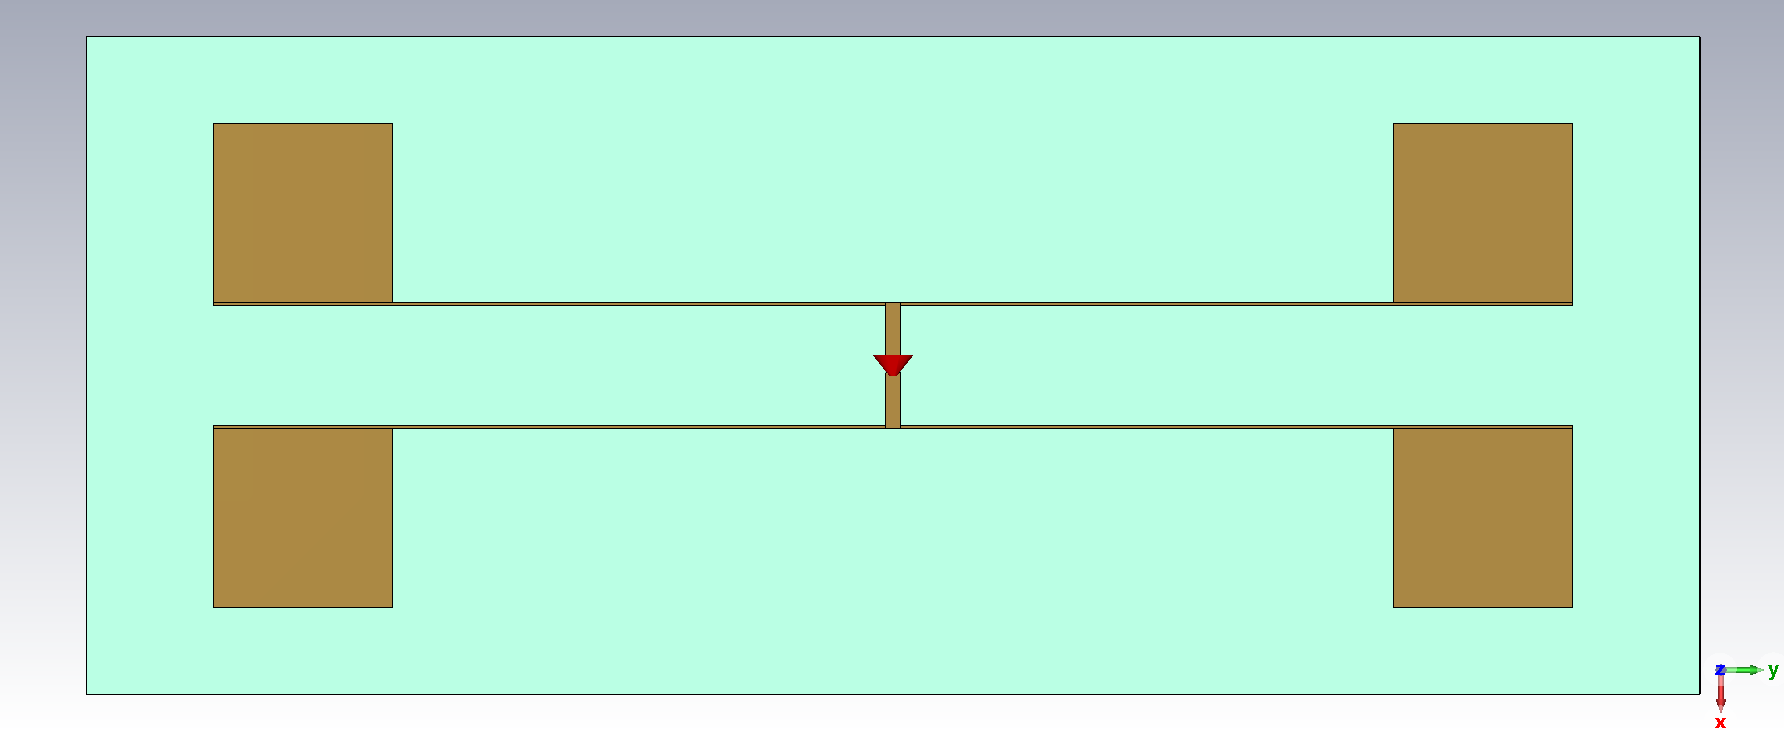
\includegraphics[width=\textwidth]{figures/H_Dipole_ref.png}
        \caption{}
        \label{fig:ref_sim}
    \end{subfigure}
    \hfill
    \begin{subfigure}[b]{0.75\textwidth}
        \centering
        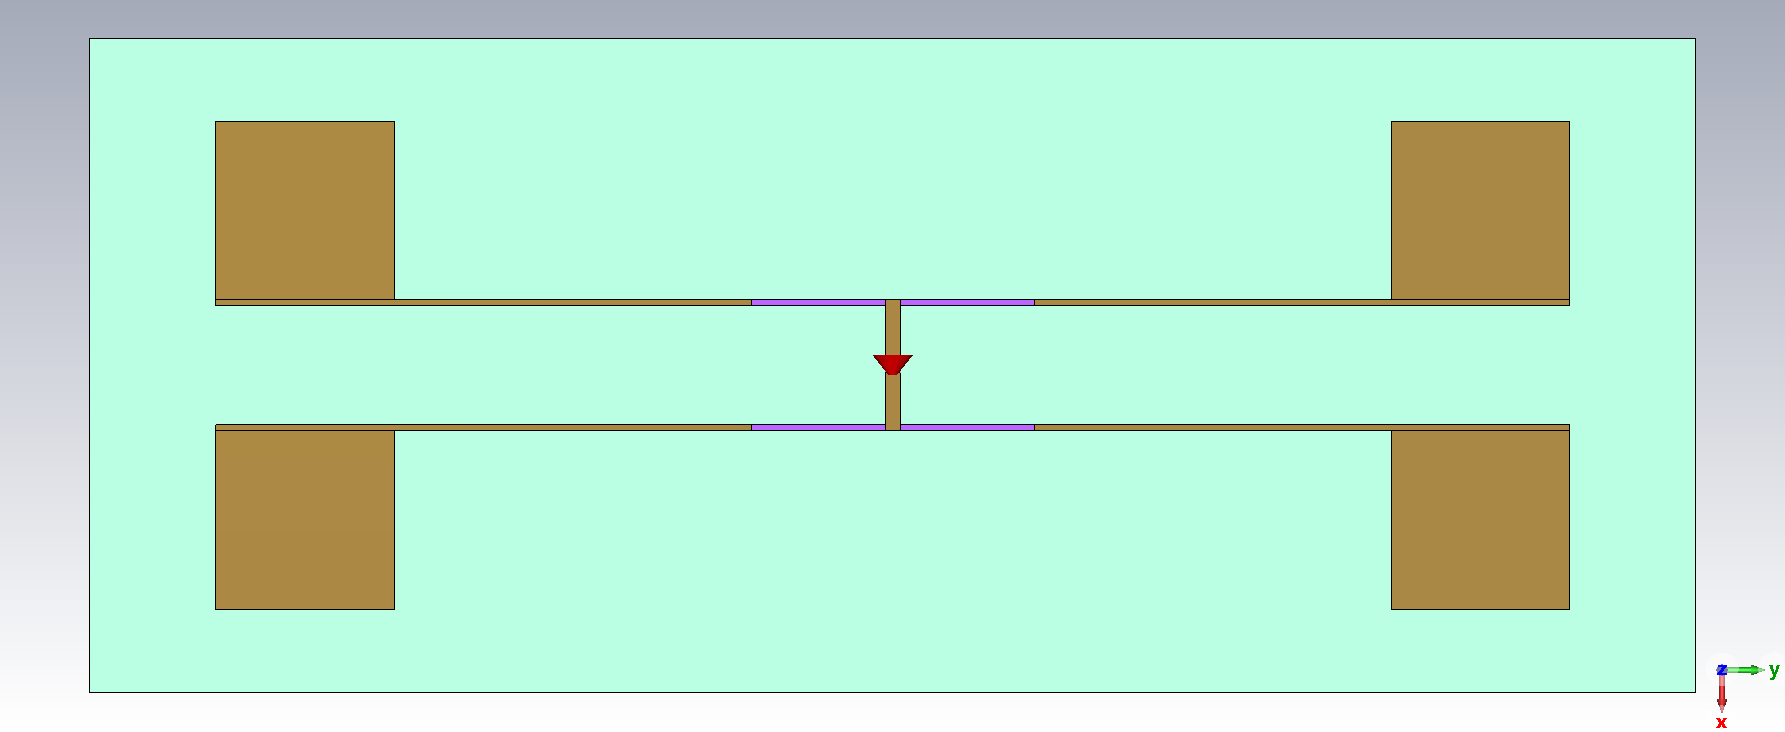
\includegraphics[width=\textwidth]{figures/H_Dipole_NiCr copy.png}
        \caption{}
        \label{fig:nicr_sim}
    \end{subfigure}
    \caption{H-Dipole antennas used in CST Studio Suite Simulations. (a) PCA used as reference for simulations. The antennas golden structure sits on top of the green substrate. In between the electrodes sits the lumped element port. (b) PCA including a NiCr-section (purple). The antennas golden structure sits on top of the green substrate. In between the electrodes sits the lumped element port.}
    \label{sim_tops}
\end{figure}

% \begin{figure}
%     \centering
%     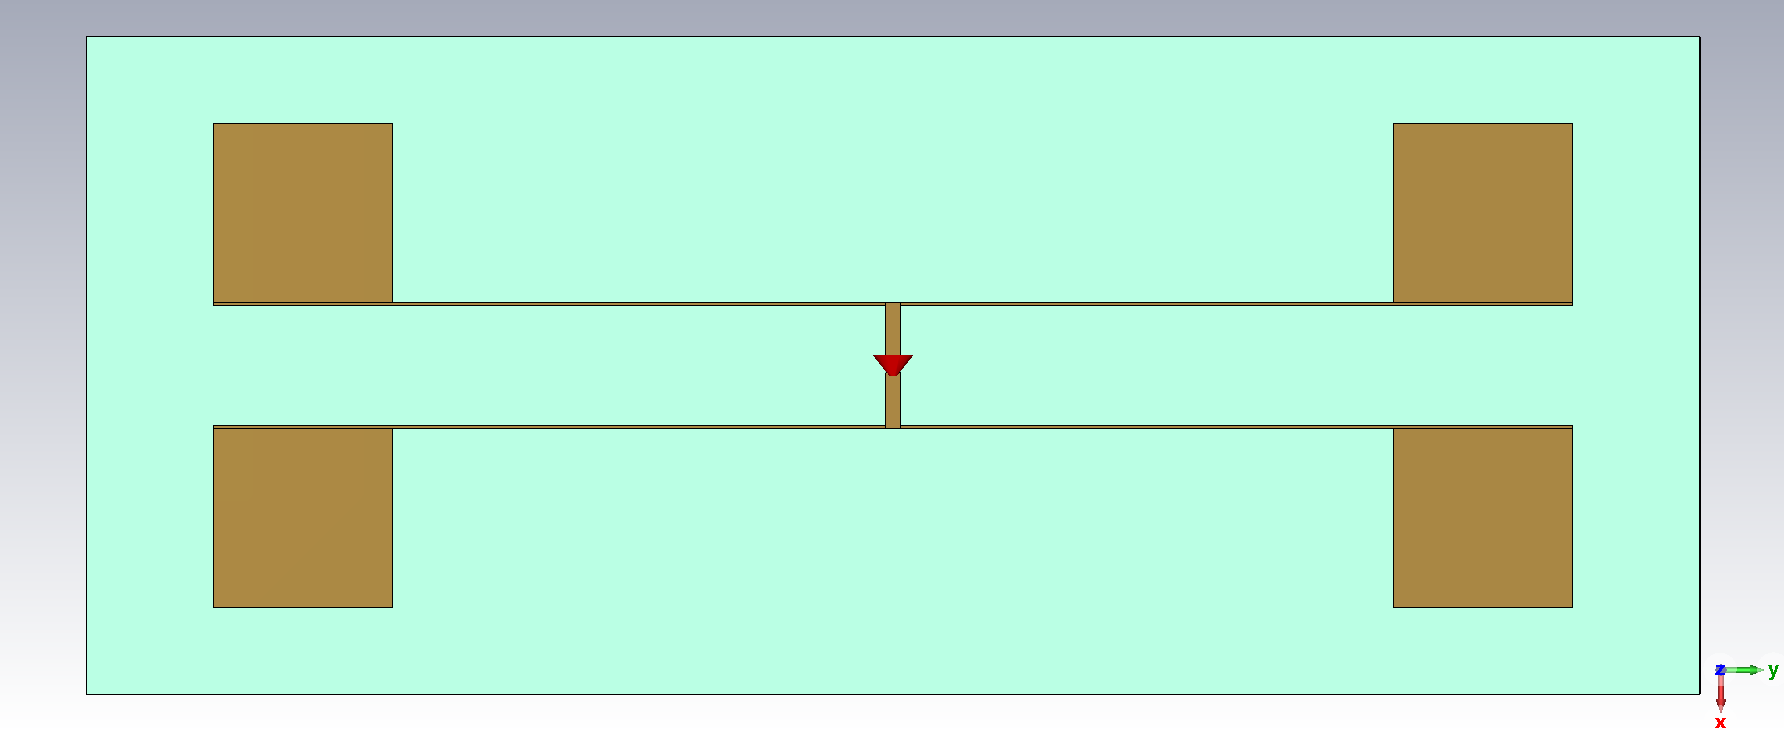
\includegraphics[width=\linewidth]{figures/H_Dipole_ref.png}
%     \caption{H-Dipole PCA used as reference for simulations in CST Studio Suite. The antennas golden structure sits on top of the green substrate. In between the electrodes sits the lumped element port.}
%     \label{ref_h_dipole_for_sim}
% \end{figure}

The H-Dipole antennas are deposited on the active photoconducting material ($\sim$ \num{1.5} \si{\micro\meter}). Below the active material sits a semi-insulating InP substrate ($\sim$ \num{500} \si{\micro\meter}). Additionally, a hyper-hemispherical silicon lense with a radius of \num{6.1} \si{\milli\meter} is attached to the substrate for efficient out-coupling of the generated THz signal. Simulating the entire structure including the silicon lense would not be feasible as too much computational power would be needed. The simulation is simplified by using a technique described in  ref. \cite{llombartTHzTimeDomainSensing2012,garufoNortonEquivalentCircuit2018}. The antenna is positioned at the air–substrate interface, where the \enquote{open add space} boundary condition is applied in CST. All other boundaries use the \enquote{open} condition, which absorbs electromagnetic radiation and mimics an infinitely extended medium. Figure \ref{fig:ref_sim} shows the topology of the reference antenna structure used in the simulation. The substrate thickness is set to at least one wavelength across all relevant frequencies. A lumped element port is used to excite the on-substrate H-dipole antenna. For reliable results, the port dimensions should be at least five times smaller than the effective wavelength. As we only investigate THz performance up to \num{1} \si{\tera\hertz}, this criterion should always be fulfilled. Simulations are performed at two distinct frequencies: \num{100} \si{\giga \hertz} and \num{1} \si{\tera\hertz}. Field monitors are set up at these distinct frequencies to capture the electromagnetic field distribution along the antenna. A monitor for the electrical field, as well as the magnetic field and surface current is implemented. 
The field distributions are simulated using the time-domain solver with a hexahedral mesh and accuracy up to \num{-30} \si{\decibel}. The time-domain solver calculates Maxwell's equations in the time-domain using finite integration technique (FIT).

\subsection{NiCr-Induced Antenna Topology}
The reference antenna topology is used to evaluate the THz performance of NiCr-induced feeding strips. Additionally to the described topology, NiCr properties are added. We start by defining NiCr's material properties. NiCr is defined as an ohmic sheet with a resistance of \num{22} \si{\ohm/sq}. 

In the reference H-Dipole topology, the deposited metal is defined as perfectly electrically conducting (PEC). This is sufficient for simulation purposes as gold can be approximated as a perfect conductor of electricity. Some part of the PEC in the antenna feeding strip is now replaced by NiCr. We start inducing the NiCr at the antenna's electrodes. This means that the longer the NiCr-strip, the closer it is to the antenna's pads. Figure \ref{fig:nicr_sim} shows an example for a H-Dipole antenna where some part of it's feeding structure is replaced by NiCr. 



\subsection{Geometries to be simulated}
The length $l_{NiCr}$ of the NiCr strip defines its resistance, as $R_{NiCr} \propto l_{NiCr}$. This is why multiple configurations have to be simulated to choose appropriate lengths for processing. 

\textbf{TODO: Table of configurations etc.}

% \begin{figure}[ht]
%     \centering
%     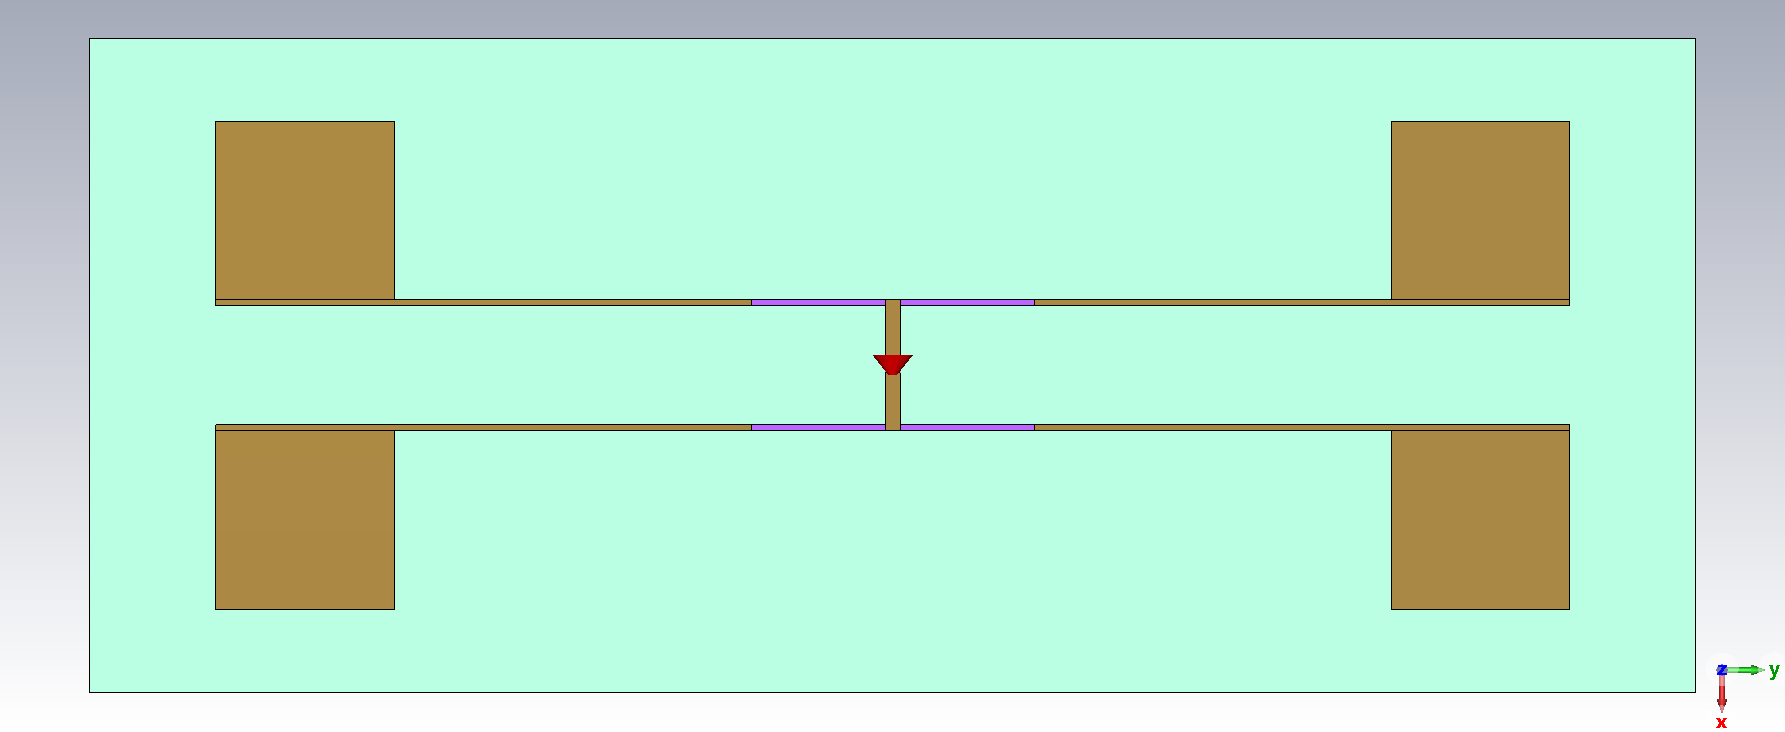
\includegraphics[width=\linewidth]{figures/H_Dipole_NiCr copy.png}
%     \caption{H-Dipole PCA including a NiCr-section (purple). The antennas golden structure sits on top of the green substrate. In between the electrodes sits the lumped element port.}
%     \label{ref_h_dipole_for_sim}
% \end{figure}
